\documentclass[twoside]{book}

% Packages required by doxygen
\usepackage{fixltx2e}
\usepackage{calc}
\usepackage{doxygen}
\usepackage[export]{adjustbox} % also loads graphicx
\usepackage{graphicx}
\usepackage[utf8]{inputenc}
\usepackage{makeidx}
\usepackage{multicol}
\usepackage{multirow}
\PassOptionsToPackage{warn}{textcomp}
\usepackage{textcomp}
\usepackage[nointegrals]{wasysym}
\usepackage[table]{xcolor}

% Font selection
\usepackage[T1]{fontenc}
\usepackage[scaled=.90]{helvet}
\usepackage{courier}
\usepackage{amssymb}
\usepackage{sectsty}
\renewcommand{\familydefault}{\sfdefault}
\allsectionsfont{%
  \fontseries{bc}\selectfont%
  \color{darkgray}%
}
\renewcommand{\DoxyLabelFont}{%
  \fontseries{bc}\selectfont%
  \color{darkgray}%
}
\newcommand{\+}{\discretionary{\mbox{\scriptsize$\hookleftarrow$}}{}{}}

% Page & text layout
\usepackage{geometry}
\geometry{%
  a4paper,%
  top=2.5cm,%
  bottom=2.5cm,%
  left=2.5cm,%
  right=2.5cm%
}
\tolerance=750
\hfuzz=15pt
\hbadness=750
\setlength{\emergencystretch}{15pt}
\setlength{\parindent}{0cm}
\setlength{\parskip}{3ex plus 2ex minus 2ex}
\makeatletter
\renewcommand{\paragraph}{%
  \@startsection{paragraph}{4}{0ex}{-1.0ex}{1.0ex}{%
    \normalfont\normalsize\bfseries\SS@parafont%
  }%
}
\renewcommand{\subparagraph}{%
  \@startsection{subparagraph}{5}{0ex}{-1.0ex}{1.0ex}{%
    \normalfont\normalsize\bfseries\SS@subparafont%
  }%
}
\makeatother

% Headers & footers
\usepackage{fancyhdr}
\pagestyle{fancyplain}
\fancyhead[LE]{\fancyplain{}{\bfseries\thepage}}
\fancyhead[CE]{\fancyplain{}{}}
\fancyhead[RE]{\fancyplain{}{\bfseries\leftmark}}
\fancyhead[LO]{\fancyplain{}{\bfseries\rightmark}}
\fancyhead[CO]{\fancyplain{}{}}
\fancyhead[RO]{\fancyplain{}{\bfseries\thepage}}
\fancyfoot[LE]{\fancyplain{}{}}
\fancyfoot[CE]{\fancyplain{}{}}
\fancyfoot[RE]{\fancyplain{}{\bfseries\scriptsize Generated by Doxygen }}
\fancyfoot[LO]{\fancyplain{}{\bfseries\scriptsize Generated by Doxygen }}
\fancyfoot[CO]{\fancyplain{}{}}
\fancyfoot[RO]{\fancyplain{}{}}
\renewcommand{\footrulewidth}{0.4pt}
\renewcommand{\chaptermark}[1]{%
  \markboth{#1}{}%
}
\renewcommand{\sectionmark}[1]{%
  \markright{\thesection\ #1}%
}

% Indices & bibliography
\usepackage{natbib}
\usepackage[titles]{tocloft}
\setcounter{tocdepth}{3}
\setcounter{secnumdepth}{5}
\makeindex

% Hyperlinks (required, but should be loaded last)
\usepackage{ifpdf}
\ifpdf
  \usepackage[pdftex,pagebackref=true]{hyperref}
\else
  \usepackage[ps2pdf,pagebackref=true]{hyperref}
\fi
\hypersetup{%
  colorlinks=true,%
  linkcolor=blue,%
  citecolor=blue,%
  unicode%
}

% Custom commands
\newcommand{\clearemptydoublepage}{%
  \newpage{\pagestyle{empty}\cleardoublepage}%
}

\usepackage{caption}
\captionsetup{labelsep=space,justification=centering,font={bf},singlelinecheck=off,skip=4pt,position=top}

%===== C O N T E N T S =====

\begin{document}

% Titlepage & ToC
\hypersetup{pageanchor=false,
             bookmarksnumbered=true,
             pdfencoding=unicode
            }
\pagenumbering{alph}
\begin{titlepage}
\vspace*{7cm}
\begin{center}%
{\Large My Project }\\
\vspace*{1cm}
{\large Generated by Doxygen 1.8.14}\\
\end{center}
\end{titlepage}
\clearemptydoublepage
\pagenumbering{roman}
\tableofcontents
\clearemptydoublepage
\pagenumbering{arabic}
\hypersetup{pageanchor=true}

%--- Begin generated contents ---
\chapter{R\+E\+A\+D\+ME}
\label{md__r_e_a_d_m_e}
\Hypertarget{md__r_e_a_d_m_e}
Hannes project

\href{https://gitlab.mpikg.mpg.de/baukmann/hannesProjekt/blob/master/html/index.html}{\tt Documentation} 
\chapter{Namespace Index}
\section{Namespace List}
Here is a list of all documented namespaces with brief descriptions\+:\begin{DoxyCompactList}
\item\contentsline{section}{\mbox{\hyperlink{namespace_hannes_o_o_p_project}{Hannes\+O\+O\+P\+Project}} \\*Description of this project }{\pageref{namespace_hannes_o_o_p_project}}{}
\end{DoxyCompactList}

\chapter{Hierarchical Index}
\section{Class Hierarchy}
This inheritance list is sorted roughly, but not completely, alphabetically\+:\begin{DoxyCompactList}
\item \contentsline{section}{O\+O\+P.\+Analysis}{\pageref{class_o_o_p_1_1_analysis}}{}
\item \contentsline{section}{O\+O\+P\+\_\+np\+Array.\+Analysis}{\pageref{class_o_o_p__np_array_1_1_analysis}}{}
\item \contentsline{section}{O\+O\+P\+\_\+np\+Array.\+Builder}{\pageref{class_o_o_p__np_array_1_1_builder}}{}
\item \contentsline{section}{O\+O\+P.\+Builder}{\pageref{class_o_o_p_1_1_builder}}{}
\item \contentsline{section}{O\+O\+P\+\_\+np\+Array.\+Cytokine}{\pageref{class_o_o_p__np_array_1_1_cytokine}}{}
\item \contentsline{section}{O\+O\+P.\+Cytokine}{\pageref{class_o_o_p_1_1_cytokine}}{}
\item \contentsline{section}{O\+O\+P.\+Glycan}{\pageref{class_o_o_p_1_1_glycan}}{}
\item \contentsline{section}{O\+O\+P\+\_\+np\+Array.\+Glycan}{\pageref{class_o_o_p__np_array_1_1_glycan}}{}
\item \contentsline{section}{O\+O\+P.\+Lectin}{\pageref{class_o_o_p_1_1_lectin}}{}
\item \contentsline{section}{O\+O\+P\+\_\+np\+Array.\+Lectin}{\pageref{class_o_o_p__np_array_1_1_lectin}}{}
\item \contentsline{section}{O\+O\+P.\+Simulation}{\pageref{class_o_o_p_1_1_simulation}}{}
\item \contentsline{section}{O\+O\+P\+\_\+np\+Array.\+Simulation}{\pageref{class_o_o_p__np_array_1_1_simulation}}{}
\item \contentsline{section}{O\+O\+P.\+Sphere}{\pageref{class_o_o_p_1_1_sphere}}{}
\begin{DoxyCompactList}
\item \contentsline{section}{O\+O\+P.\+Bead}{\pageref{class_o_o_p_1_1_bead}}{}
\item \contentsline{section}{O\+O\+P.\+Decoder\+Cell}{\pageref{class_o_o_p_1_1_decoder_cell}}{}
\end{DoxyCompactList}
\item \contentsline{section}{O\+O\+P\+\_\+np\+Array.\+Sphere}{\pageref{class_o_o_p__np_array_1_1_sphere}}{}
\begin{DoxyCompactList}
\item \contentsline{section}{O\+O\+P\+\_\+np\+Array.\+Bead}{\pageref{class_o_o_p__np_array_1_1_bead}}{}
\item \contentsline{section}{O\+O\+P\+\_\+np\+Array.\+Decoder\+Cell}{\pageref{class_o_o_p__np_array_1_1_decoder_cell}}{}
\end{DoxyCompactList}
\item \contentsline{section}{O\+O\+P\+\_\+np\+Array.\+Well}{\pageref{class_o_o_p__np_array_1_1_well}}{}
\begin{DoxyCompactList}
\item \contentsline{section}{O\+O\+P\+\_\+np\+Array.\+Well\+\_\+list}{\pageref{class_o_o_p__np_array_1_1_well__list}}{}
\item \contentsline{section}{O\+O\+P\+\_\+np\+Array.\+Well\+\_\+np\+Array}{\pageref{class_o_o_p__np_array_1_1_well__np_array}}{}
\end{DoxyCompactList}
\item \contentsline{section}{O\+O\+P.\+Well}{\pageref{class_o_o_p_1_1_well}}{}
\end{DoxyCompactList}

\chapter{Class Index}
\section{Class List}
Here are the classes, structs, unions and interfaces with brief descriptions\+:\begin{DoxyCompactList}
\item\contentsline{section}{\mbox{\hyperlink{class_o_o_p_1_1_cell}{O\+O\+P.\+Cell}} \\*Dokumentation for class \mbox{\hyperlink{class_o_o_p_1_1_cell}{Cell}} }{\pageref{class_o_o_p_1_1_cell}}{}
\item\contentsline{section}{\mbox{\hyperlink{class_o_o_p_1_1_decoder_cell}{O\+O\+P.\+Decoder\+Cell}} }{\pageref{class_o_o_p_1_1_decoder_cell}}{}
\item\contentsline{section}{\mbox{\hyperlink{class_o_o_p_1_1_encoder_cell}{O\+O\+P.\+Encoder\+Cell}} }{\pageref{class_o_o_p_1_1_encoder_cell}}{}
\item\contentsline{section}{\mbox{\hyperlink{class_o_o_p_1_1_glycan}{O\+O\+P.\+Glycan}} }{\pageref{class_o_o_p_1_1_glycan}}{}
\item\contentsline{section}{\mbox{\hyperlink{class_o_o_p_1_1_lectin}{O\+O\+P.\+Lectin}} }{\pageref{class_o_o_p_1_1_lectin}}{}
\item\contentsline{section}{\mbox{\hyperlink{classprototype_1_1_object_factory}{prototype.\+Object\+Factory}} }{\pageref{classprototype_1_1_object_factory}}{}
\item\contentsline{section}{\mbox{\hyperlink{classprototype_1_1_prototype}{prototype.\+Prototype}} }{\pageref{classprototype_1_1_prototype}}{}
\item\contentsline{section}{\mbox{\hyperlink{classprototype_1_1_type1}{prototype.\+Type1}} }{\pageref{classprototype_1_1_type1}}{}
\item\contentsline{section}{\mbox{\hyperlink{classprototype_1_1_type2}{prototype.\+Type2}} }{\pageref{classprototype_1_1_type2}}{}
\end{DoxyCompactList}

\chapter{Namespace Documentation}
\hypertarget{namespaceawesome3_d}{}\section{awesome3D Namespace Reference}
\label{namespaceawesome3_d}\index{awesome3D@{awesome3D}}
\subsection*{Functions}
\begin{DoxyCompactItemize}
\item 
def \mbox{\hyperlink{namespaceawesome3_d_a8dbde731a58e2a410a00a8b710f675dd}{Gen\+\_\+\+Rand\+Line}} (length, dims=2)
\item 
\mbox{\Hypertarget{namespaceawesome3_d_a3880bce8144e84df6f930e519f8aaf4b}\label{namespaceawesome3_d_a3880bce8144e84df6f930e519f8aaf4b}} 
def {\bfseries update\+\_\+lines} (num, data\+Lines, lines)
\end{DoxyCompactItemize}
\subsection*{Variables}
\begin{DoxyCompactItemize}
\item 
\mbox{\Hypertarget{namespaceawesome3_d_a1d67360c21020aa16682a83c2728f039}\label{namespaceawesome3_d_a1d67360c21020aa16682a83c2728f039}} 
{\bfseries fig} = plt.\+figure()
\item 
\mbox{\Hypertarget{namespaceawesome3_d_a1924ab2ef7c8b99f6dbaa5abe2fb6f7b}\label{namespaceawesome3_d_a1924ab2ef7c8b99f6dbaa5abe2fb6f7b}} 
{\bfseries ax} = p3.\+Axes3D(fig)
\item 
\mbox{\Hypertarget{namespaceawesome3_d_a4b315f767d2e877640adbe6f9b4e2a67}\label{namespaceawesome3_d_a4b315f767d2e877640adbe6f9b4e2a67}} 
list {\bfseries data} = \mbox{[}\mbox{\hyperlink{namespaceawesome3_d_a8dbde731a58e2a410a00a8b710f675dd}{Gen\+\_\+\+Rand\+Line}}(25, 3) for index in range(50)\mbox{]}
\item 
\mbox{\Hypertarget{namespaceawesome3_d_a6eb83efe0d9acac5432efdb18bba939d}\label{namespaceawesome3_d_a6eb83efe0d9acac5432efdb18bba939d}} 
list {\bfseries lines} = \mbox{[}ax.\+plot(dat\mbox{[}0, 0\+:1\mbox{]}, dat\mbox{[}1, 0\+:1\mbox{]}, dat\mbox{[}2, 0\+:1\mbox{]})\mbox{[}0\mbox{]} for dat in data\mbox{]}
\item 
{\bfseries line\+\_\+ani}
\end{DoxyCompactItemize}


\subsection{Detailed Description}
\begin{DoxyVerb}============
3D animation
============

A simple example of an animated plot... In 3D!
\end{DoxyVerb}
 

\subsection{Function Documentation}
\mbox{\Hypertarget{namespaceawesome3_d_a8dbde731a58e2a410a00a8b710f675dd}\label{namespaceawesome3_d_a8dbde731a58e2a410a00a8b710f675dd}} 
\index{awesome3D@{awesome3D}!Gen\+\_\+\+Rand\+Line@{Gen\+\_\+\+Rand\+Line}}
\index{Gen\+\_\+\+Rand\+Line@{Gen\+\_\+\+Rand\+Line}!awesome3D@{awesome3D}}
\subsubsection{\texorpdfstring{Gen\+\_\+\+Rand\+Line()}{Gen\_RandLine()}}
{\footnotesize\ttfamily def awesome3\+D.\+Gen\+\_\+\+Rand\+Line (\begin{DoxyParamCaption}\item[{}]{length,  }\item[{}]{dims = {\ttfamily 2} }\end{DoxyParamCaption})}

\begin{DoxyVerb}Create a line using a random walk algorithm

length is the number of points for the line.
dims is the number of dimensions the line has.
\end{DoxyVerb}
 

\subsection{Variable Documentation}
\mbox{\Hypertarget{namespaceawesome3_d_af81b21dee31a4d9e3517281959dc0f13}\label{namespaceawesome3_d_af81b21dee31a4d9e3517281959dc0f13}} 
\index{awesome3D@{awesome3D}!line\+\_\+ani@{line\+\_\+ani}}
\index{line\+\_\+ani@{line\+\_\+ani}!awesome3D@{awesome3D}}
\subsubsection{\texorpdfstring{line\+\_\+ani}{line\_ani}}
{\footnotesize\ttfamily awesome3\+D.\+line\+\_\+ani}

{\bfseries Initial value\+:}
\begin{DoxyCode}
1 =  animation.FuncAnimation(fig, update\_lines, 25, fargs=(data, lines),
2                                    interval=50, blit=\textcolor{keyword}{False})
\end{DoxyCode}

\hypertarget{namespace_hannes_o_o_p_project}{}\section{Hannes\+O\+O\+P\+Project Namespace Reference}
\label{namespace_hannes_o_o_p_project}\index{Hannes\+O\+O\+P\+Project@{Hannes\+O\+O\+P\+Project}}


Description of this project.  




\subsection{Detailed Description}
Description of this project. 

\subsection*{Ueberschift! }
\chapter{Class Documentation}
\hypertarget{class_o_o_p_1_1_cell}{}\section{O\+O\+P.\+Cell Class Reference}
\label{class_o_o_p_1_1_cell}\index{O\+O\+P.\+Cell@{O\+O\+P.\+Cell}}


Dokumentation for class \mbox{\hyperlink{class_o_o_p_1_1_cell}{Cell}}.  


Inheritance diagram for O\+O\+P.\+Cell\+:\begin{figure}[H]
\begin{center}
\leavevmode
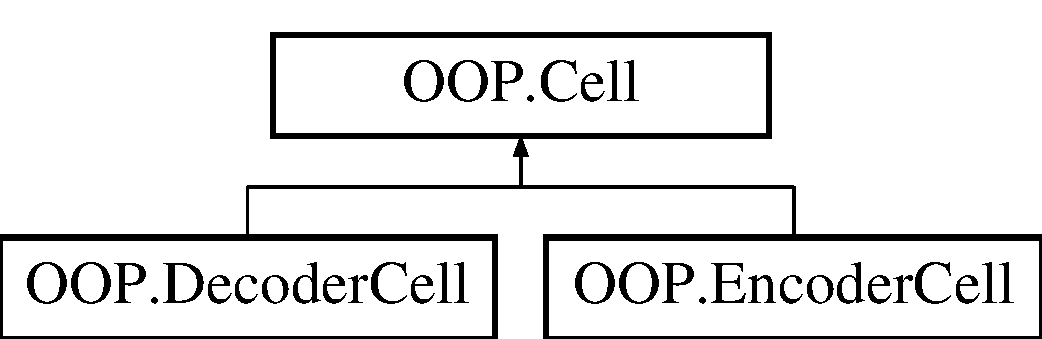
\includegraphics[height=2.000000cm]{class_o_o_p_1_1_cell}
\end{center}
\end{figure}
\subsection*{Public Member Functions}
\begin{DoxyCompactItemize}
\item 
def \mbox{\hyperlink{class_o_o_p_1_1_cell_ab1a324a4456c36a49868ba26cd76eb39}{\+\_\+\+\_\+init\+\_\+\+\_\+}} (self)
\begin{DoxyCompactList}\small\item\em The constructor. \end{DoxyCompactList}\item 
\mbox{\Hypertarget{class_o_o_p_1_1_cell_a43bf87982f526ebdcf3334ab9d9038fd}\label{class_o_o_p_1_1_cell_a43bf87982f526ebdcf3334ab9d9038fd}} 
def {\bfseries random\+Walk2D} (self, n)
\item 
\mbox{\Hypertarget{class_o_o_p_1_1_cell_ade9b333c2663aed86972a68048c7abb4}\label{class_o_o_p_1_1_cell_ade9b333c2663aed86972a68048c7abb4}} 
def {\bfseries random\+Walk3D} (self)
\end{DoxyCompactItemize}


\subsection{Detailed Description}
Dokumentation for class \mbox{\hyperlink{class_o_o_p_1_1_cell}{Cell}}. 



\subsection{Constructor \& Destructor Documentation}
\mbox{\Hypertarget{class_o_o_p_1_1_cell_ab1a324a4456c36a49868ba26cd76eb39}\label{class_o_o_p_1_1_cell_ab1a324a4456c36a49868ba26cd76eb39}} 
\index{O\+O\+P\+::\+Cell@{O\+O\+P\+::\+Cell}!\+\_\+\+\_\+init\+\_\+\+\_\+@{\+\_\+\+\_\+init\+\_\+\+\_\+}}
\index{\+\_\+\+\_\+init\+\_\+\+\_\+@{\+\_\+\+\_\+init\+\_\+\+\_\+}!O\+O\+P\+::\+Cell@{O\+O\+P\+::\+Cell}}
\subsubsection{\texorpdfstring{\+\_\+\+\_\+init\+\_\+\+\_\+()}{\_\_init\_\_()}}
{\footnotesize\ttfamily def O\+O\+P.\+Cell.\+\_\+\+\_\+init\+\_\+\+\_\+ (\begin{DoxyParamCaption}\item[{}]{self }\end{DoxyParamCaption})}



The constructor. 



The documentation for this class was generated from the following file\+:\begin{DoxyCompactItemize}
\item 
O\+O\+P.\+py\end{DoxyCompactItemize}

\hypertarget{class_o_o_p_1_1_decoder_cell}{}\section{O\+O\+P.\+Decoder\+Cell Class Reference}
\label{class_o_o_p_1_1_decoder_cell}\index{O\+O\+P.\+Decoder\+Cell@{O\+O\+P.\+Decoder\+Cell}}
Inheritance diagram for O\+O\+P.\+Decoder\+Cell\+:\begin{figure}[H]
\begin{center}
\leavevmode
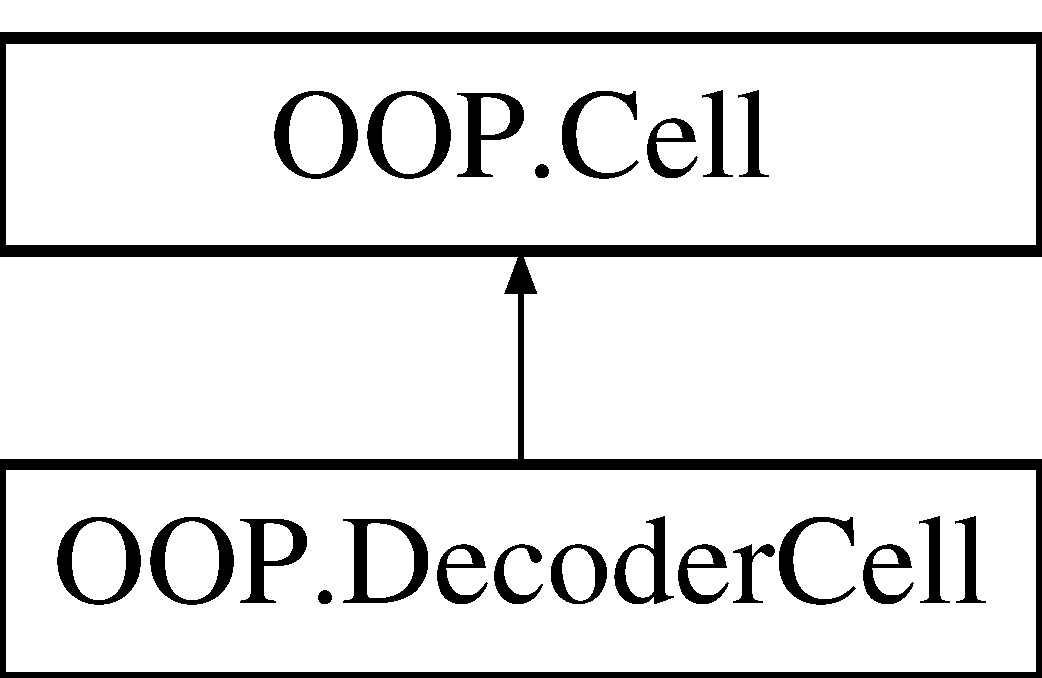
\includegraphics[height=2.000000cm]{class_o_o_p_1_1_decoder_cell}
\end{center}
\end{figure}
\subsection*{Public Member Functions}
\begin{DoxyCompactItemize}
\item 
\mbox{\Hypertarget{class_o_o_p_1_1_decoder_cell_ae361486a3a0bfd2be707a6fb6fc76222}\label{class_o_o_p_1_1_decoder_cell_ae361486a3a0bfd2be707a6fb6fc76222}} 
def {\bfseries binding} (self, encoder\+Cell)
\item 
\mbox{\Hypertarget{class_o_o_p_1_1_decoder_cell_a08d8eafb492ffde3dc5d461997faf206}\label{class_o_o_p_1_1_decoder_cell_a08d8eafb492ffde3dc5d461997faf206}} 
def {\bfseries get\+All\+Lectins} (self)
\item 
\mbox{\Hypertarget{class_o_o_p_1_1_decoder_cell_a8c5a2b96eb3d7fda5ec0ae2e6b3bb3e3}\label{class_o_o_p_1_1_decoder_cell_a8c5a2b96eb3d7fda5ec0ae2e6b3bb3e3}} 
def {\bfseries show\+Density} (self)
\item 
\mbox{\Hypertarget{class_o_o_p_1_1_decoder_cell_af8a8eee539e3b3c83f5d7ea550a5eb21}\label{class_o_o_p_1_1_decoder_cell_af8a8eee539e3b3c83f5d7ea550a5eb21}} 
def {\bfseries cytokine\+Expression} (self)
\end{DoxyCompactItemize}


The documentation for this class was generated from the following file\+:\begin{DoxyCompactItemize}
\item 
O\+O\+P.\+py\end{DoxyCompactItemize}

\hypertarget{class_o_o_p_1_1_encoder_cell}{}\section{O\+O\+P.\+Encoder\+Cell Class Reference}
\label{class_o_o_p_1_1_encoder_cell}\index{O\+O\+P.\+Encoder\+Cell@{O\+O\+P.\+Encoder\+Cell}}
Inheritance diagram for O\+O\+P.\+Encoder\+Cell\+:\begin{figure}[H]
\begin{center}
\leavevmode
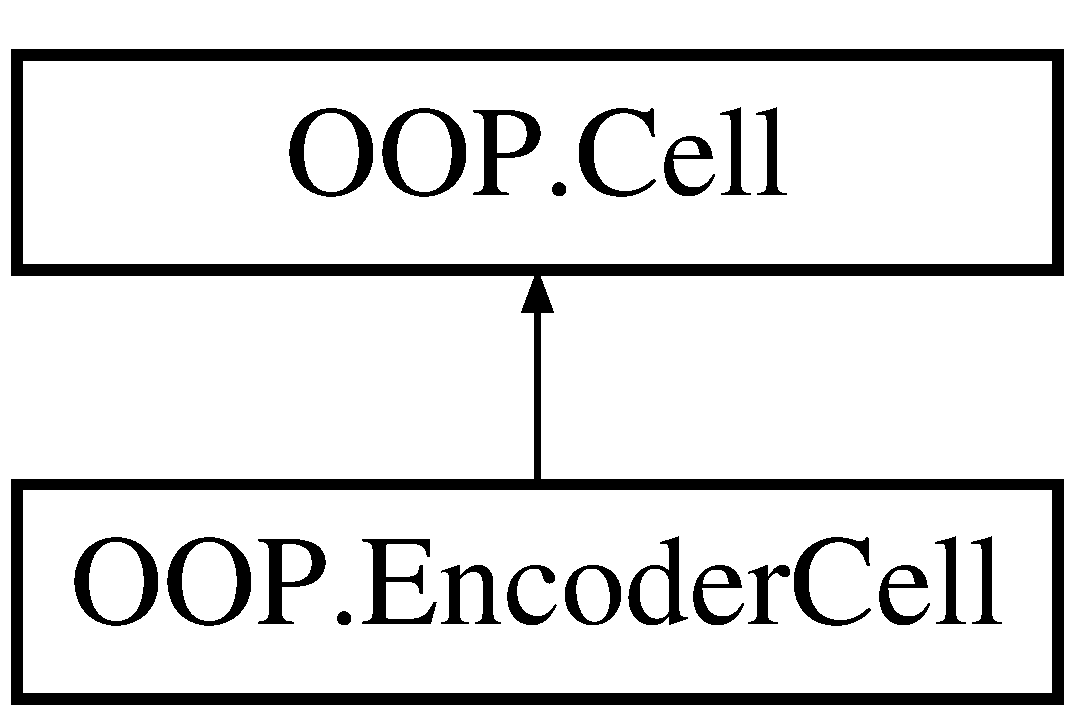
\includegraphics[height=2.000000cm]{class_o_o_p_1_1_encoder_cell}
\end{center}
\end{figure}
\subsection*{Additional Inherited Members}


The documentation for this class was generated from the following file\+:\begin{DoxyCompactItemize}
\item 
O\+O\+P.\+py\end{DoxyCompactItemize}

\hypertarget{class_o_o_p_1_1_glycan}{}\section{O\+O\+P.\+Glycan Class Reference}
\label{class_o_o_p_1_1_glycan}\index{O\+O\+P.\+Glycan@{O\+O\+P.\+Glycan}}


The documentation for this class was generated from the following file\+:\begin{DoxyCompactItemize}
\item 
O\+O\+P.\+py\end{DoxyCompactItemize}

\hypertarget{class_o_o_p_1_1_lectin}{}\section{O\+O\+P.\+Lectin Class Reference}
\label{class_o_o_p_1_1_lectin}\index{O\+O\+P.\+Lectin@{O\+O\+P.\+Lectin}}


The documentation for this class was generated from the following file\+:\begin{DoxyCompactItemize}
\item 
O\+O\+P.\+py\end{DoxyCompactItemize}

\hypertarget{classprototype_1_1_object_factory}{}\section{prototype.\+Object\+Factory Class Reference}
\label{classprototype_1_1_object_factory}\index{prototype.\+Object\+Factory@{prototype.\+Object\+Factory}}
\subsection*{Static Public Member Functions}
\begin{DoxyCompactItemize}
\item 
\mbox{\Hypertarget{classprototype_1_1_object_factory_ab9e8031330594af772d0e464a97f639f}\label{classprototype_1_1_object_factory_ab9e8031330594af772d0e464a97f639f}} 
def {\bfseries initialize} ()
\item 
\mbox{\Hypertarget{classprototype_1_1_object_factory_a7d9693c4c85b69eb1cbd3e837160eefb}\label{classprototype_1_1_object_factory_a7d9693c4c85b69eb1cbd3e837160eefb}} 
def {\bfseries get\+Type1\+Value1} ()
\item 
\mbox{\Hypertarget{classprototype_1_1_object_factory_a714d45fccd5421d4302c2941f409e534}\label{classprototype_1_1_object_factory_a714d45fccd5421d4302c2941f409e534}} 
def {\bfseries get\+Type1\+Value2} ()
\item 
\mbox{\Hypertarget{classprototype_1_1_object_factory_a7d3f3ef590862a071009ba0cca5c844c}\label{classprototype_1_1_object_factory_a7d3f3ef590862a071009ba0cca5c844c}} 
def {\bfseries get\+Type2\+Value1} ()
\item 
\mbox{\Hypertarget{classprototype_1_1_object_factory_a044abe63bccc47babe3aaa9cee223e3d}\label{classprototype_1_1_object_factory_a044abe63bccc47babe3aaa9cee223e3d}} 
def {\bfseries get\+Type2\+Value2} ()
\end{DoxyCompactItemize}


\subsection{Detailed Description}
\begin{DoxyVerb}Manages prototypes.
Static factory, that encapsulates prototype
initialization and then allows instatiation
of the classes from these prototypes.
\end{DoxyVerb}
 

The documentation for this class was generated from the following file\+:\begin{DoxyCompactItemize}
\item 
prototype.\+py\end{DoxyCompactItemize}

\hypertarget{classprototype_1_1_prototype}{}\section{prototype.\+Prototype Class Reference}
\label{classprototype_1_1_prototype}\index{prototype.\+Prototype@{prototype.\+Prototype}}
Inheritance diagram for prototype.\+Prototype\+:\begin{figure}[H]
\begin{center}
\leavevmode
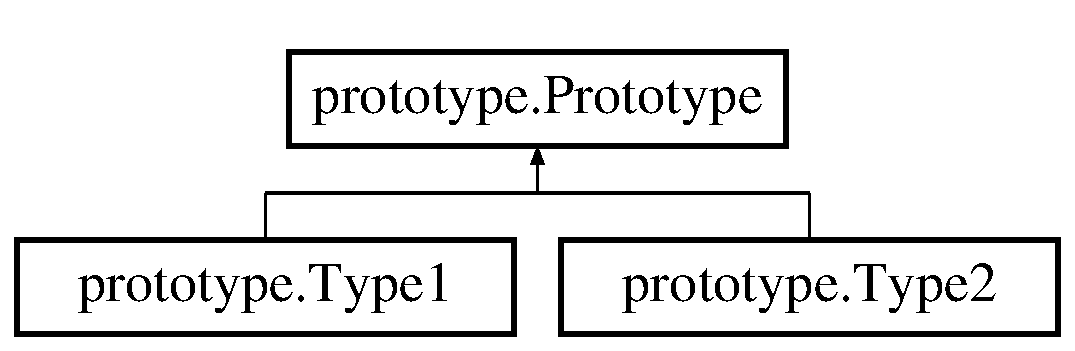
\includegraphics[height=2.000000cm]{classprototype_1_1_prototype}
\end{center}
\end{figure}
\subsection*{Public Member Functions}
\begin{DoxyCompactItemize}
\item 
\mbox{\Hypertarget{classprototype_1_1_prototype_aa9ace38c2c392b1770e0d421e7435740}\label{classprototype_1_1_prototype_aa9ace38c2c392b1770e0d421e7435740}} 
def {\bfseries clone} (self)
\item 
\mbox{\Hypertarget{classprototype_1_1_prototype_a9a805e5c947324964a491654407512cc}\label{classprototype_1_1_prototype_a9a805e5c947324964a491654407512cc}} 
def {\bfseries get\+Type} (self)
\item 
\mbox{\Hypertarget{classprototype_1_1_prototype_aa41392dd1441dcca9942f61b6980d958}\label{classprototype_1_1_prototype_aa41392dd1441dcca9942f61b6980d958}} 
def {\bfseries get\+Value} (self)
\end{DoxyCompactItemize}


\subsection{Detailed Description}
\begin{DoxyVerb}Object, that can be cloned.
This is just a base class, so the clone() method
is not implemented. But all subclasses have to
override it.
\end{DoxyVerb}
 

The documentation for this class was generated from the following file\+:\begin{DoxyCompactItemize}
\item 
prototype.\+py\end{DoxyCompactItemize}

\hypertarget{classprototype_1_1_type1}{}\section{prototype.\+Type1 Class Reference}
\label{classprototype_1_1_type1}\index{prototype.\+Type1@{prototype.\+Type1}}
Inheritance diagram for prototype.\+Type1\+:\begin{figure}[H]
\begin{center}
\leavevmode
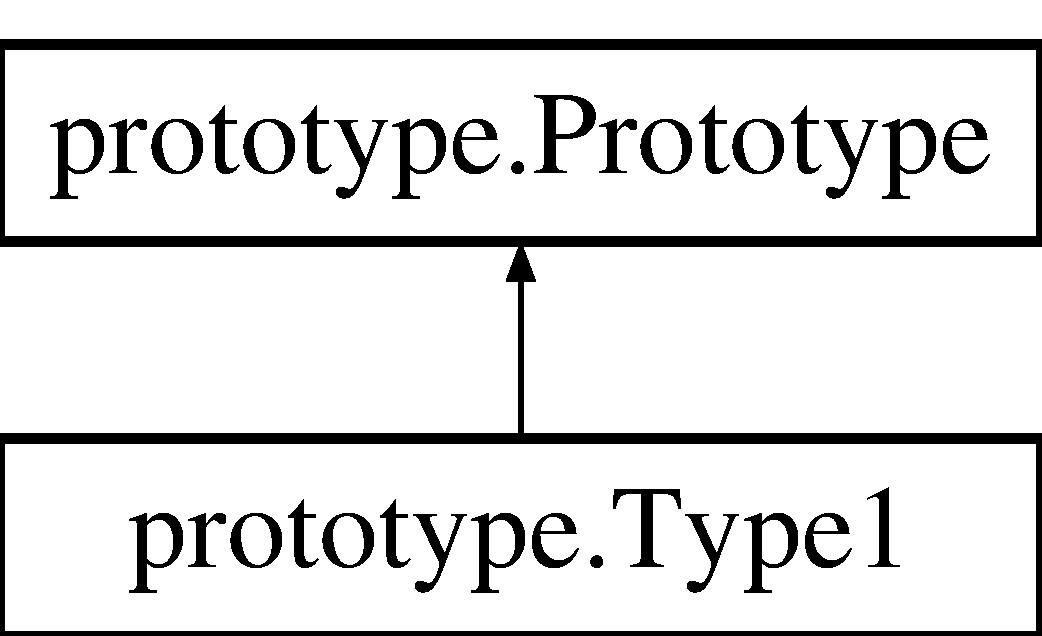
\includegraphics[height=2.000000cm]{classprototype_1_1_type1}
\end{center}
\end{figure}
\subsection*{Public Member Functions}
\begin{DoxyCompactItemize}
\item 
\mbox{\Hypertarget{classprototype_1_1_type1_aa9d24cececd5e64697e9b0869fc7be37}\label{classprototype_1_1_type1_aa9d24cececd5e64697e9b0869fc7be37}} 
def {\bfseries \+\_\+\+\_\+init\+\_\+\+\_\+} (self, number)
\item 
\mbox{\Hypertarget{classprototype_1_1_type1_a14acd74005626171d11916bce618a421}\label{classprototype_1_1_type1_a14acd74005626171d11916bce618a421}} 
def {\bfseries clone} (self)
\end{DoxyCompactItemize}


\subsection{Detailed Description}
\begin{DoxyVerb}Concrete prototype.

Implementation of Prototype. Important part is the
clone() method.
\end{DoxyVerb}
 

The documentation for this class was generated from the following file\+:\begin{DoxyCompactItemize}
\item 
prototype.\+py\end{DoxyCompactItemize}

\hypertarget{classprototype_1_1_type2}{}\section{prototype.\+Type2 Class Reference}
\label{classprototype_1_1_type2}\index{prototype.\+Type2@{prototype.\+Type2}}
Inheritance diagram for prototype.\+Type2\+:\begin{figure}[H]
\begin{center}
\leavevmode
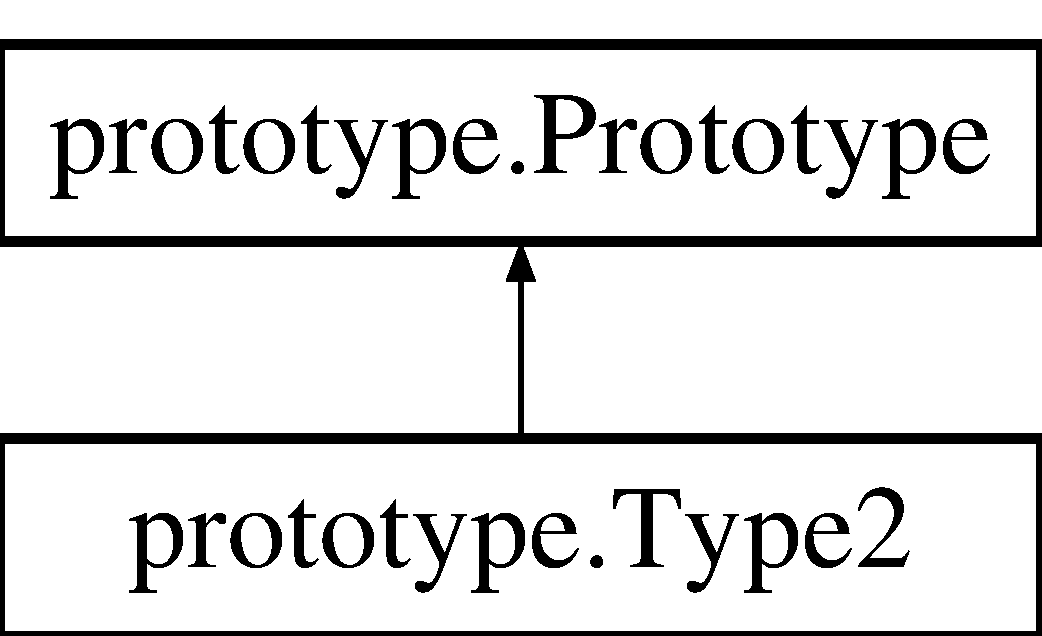
\includegraphics[height=2.000000cm]{classprototype_1_1_type2}
\end{center}
\end{figure}
\subsection*{Public Member Functions}
\begin{DoxyCompactItemize}
\item 
\mbox{\Hypertarget{classprototype_1_1_type2_ac5fc947194ea1fc853a77f7824199bf8}\label{classprototype_1_1_type2_ac5fc947194ea1fc853a77f7824199bf8}} 
def {\bfseries \+\_\+\+\_\+init\+\_\+\+\_\+} (self, number)
\item 
\mbox{\Hypertarget{classprototype_1_1_type2_aaca5eda564d17f7ec59cee14dc196626}\label{classprototype_1_1_type2_aaca5eda564d17f7ec59cee14dc196626}} 
def {\bfseries clone} (self)
\end{DoxyCompactItemize}


\subsection{Detailed Description}
\begin{DoxyVerb}Concrete prototype. \end{DoxyVerb}
 

The documentation for this class was generated from the following file\+:\begin{DoxyCompactItemize}
\item 
prototype.\+py\end{DoxyCompactItemize}

%--- End generated contents ---

% Index
\backmatter
\newpage
\phantomsection
\clearemptydoublepage
\addcontentsline{toc}{chapter}{Index}
\printindex

\end{document}
